\documentclass[12pt, a4paper]{article}

\usepackage[hmargin=2.5cm, vmargin=2cm]{geometry}
\usepackage{amsthm, amssymb, mathtools, yhmath, graphicx}
\usepackage{fontspec, type1cm, titlesec, titling, fancyhdr, tabularx}
\usepackage{color}
\usepackage{unicode-math}
\usepackage{float}
\usepackage{hhline}
\usepackage{comment}
\usepackage{siunitx}
\usepackage{csvsimple}
\usepackage{subcaption}

\usepackage[CheckSingle, CJKmath]{xeCJK}
\usepackage{CJKulem}
\usepackage{enumitem}
\usepackage{tikz}
\usepackage[siunitx]{circuitikz}
\usepackage{wrapfig}
%\setCJKmainfont[BoldFont=cwTex Q Hei]{cwTex Q Ming}
%\setCJKsansfont[BoldFont=cwTex Q Hei]{cwTex Q Ming}
%\setCJKmonofont[BoldFont=cwTex Q Hei]{cwTex Q Ming}
\setCJKmainfont[BoldFont=cwTeX Q Hei]{cwTeX Q Ming}

\def\normalsize{\fontsize{12}{18}\selectfont}
\def\large{\fontsize{14}{21}\selectfont}
\def\Large{\fontsize{16}{24}\selectfont}
\def\LARGE{\fontsize{18}{27}\selectfont}
\def\huge{\fontsize{20}{30}\selectfont}

%\titleformat{\section}{\bf\Large}{\arabic{section}}{24pt}{}
%\titleformat{\subsection}{\large}{\arabic{subsection}.}{12pt}{}
%\titlespacing*{\subsection}{0pt}{0pt}{1.5ex}

\parindent=24pt

\DeclarePairedDelimiter{\abs}{\lvert}{\rvert}
\DeclarePairedDelimiter{\norm}{\lVert}{\rVert}
\DeclarePairedDelimiter{\inpd}{\langle}{\rangle}
\DeclarePairedDelimiter{\ceil}{\lceil}{\rceil}
\DeclarePairedDelimiter{\floor}{\lfloor}{\rfloor}

\newcommand{\unit}[1]{\:(\text{#1})}
\newcommand{\df}[1]{\mathop{}\!\mathrm{d^#1}}
\newcommand{\img}{\mathrm{i}}

\title{ \bf {\Huge 電子電路實驗7:雙極非線性元件特性曲線之簡單測量}\\ 實驗結報}
\author{B02901178 江誠敏}

\begin{document}

\maketitle


\section{實驗結果}
\subsection{\SI{5.1}\kohm}
\begin{figure}[H]
  \centering
  \begin{subfigure}[b]{0.45\textwidth}
    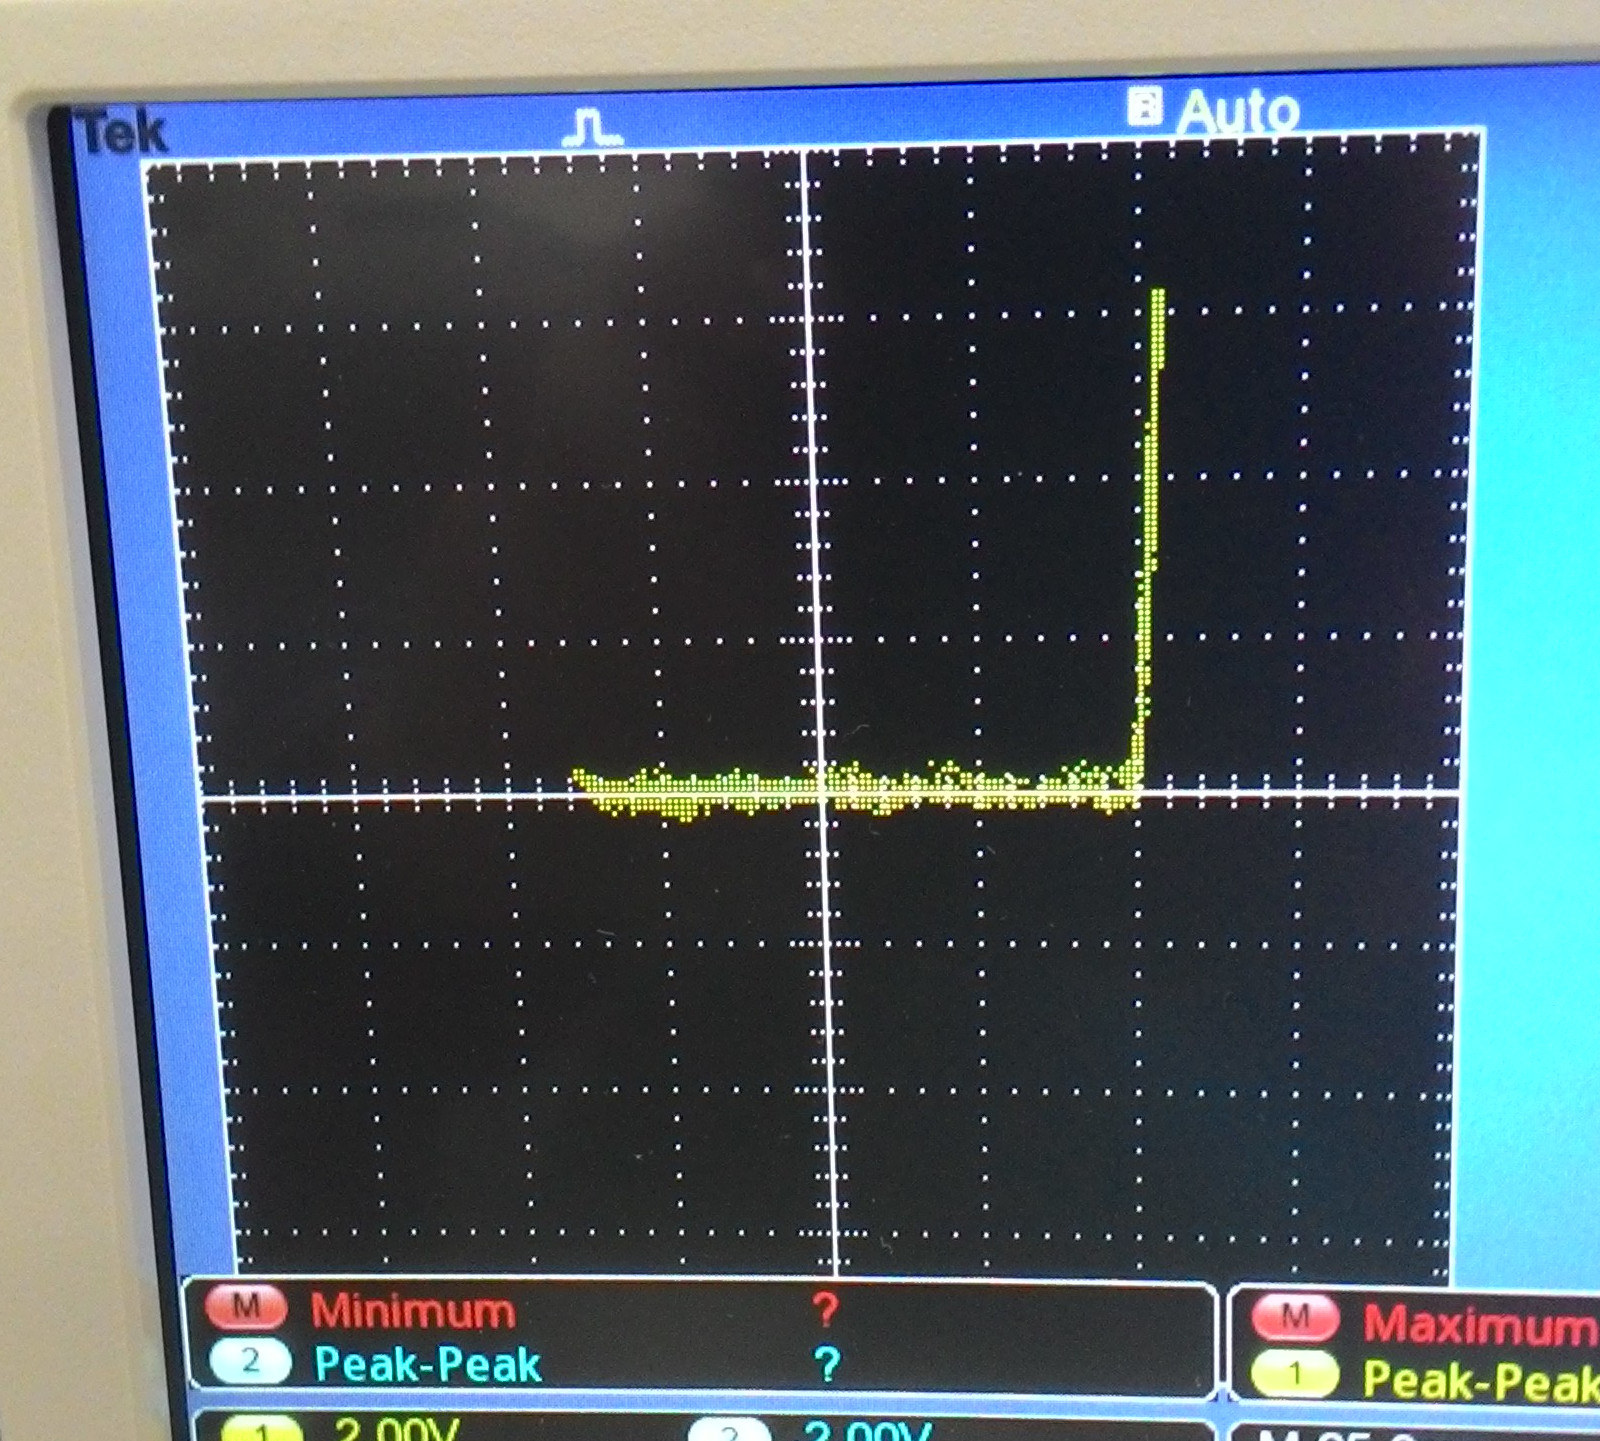
\includegraphics[width=1\textwidth]{img/P1.jpg}
    \caption{Si}
  \end{subfigure}
  ~
  \begin{subfigure}[b]{0.45\textwidth}
    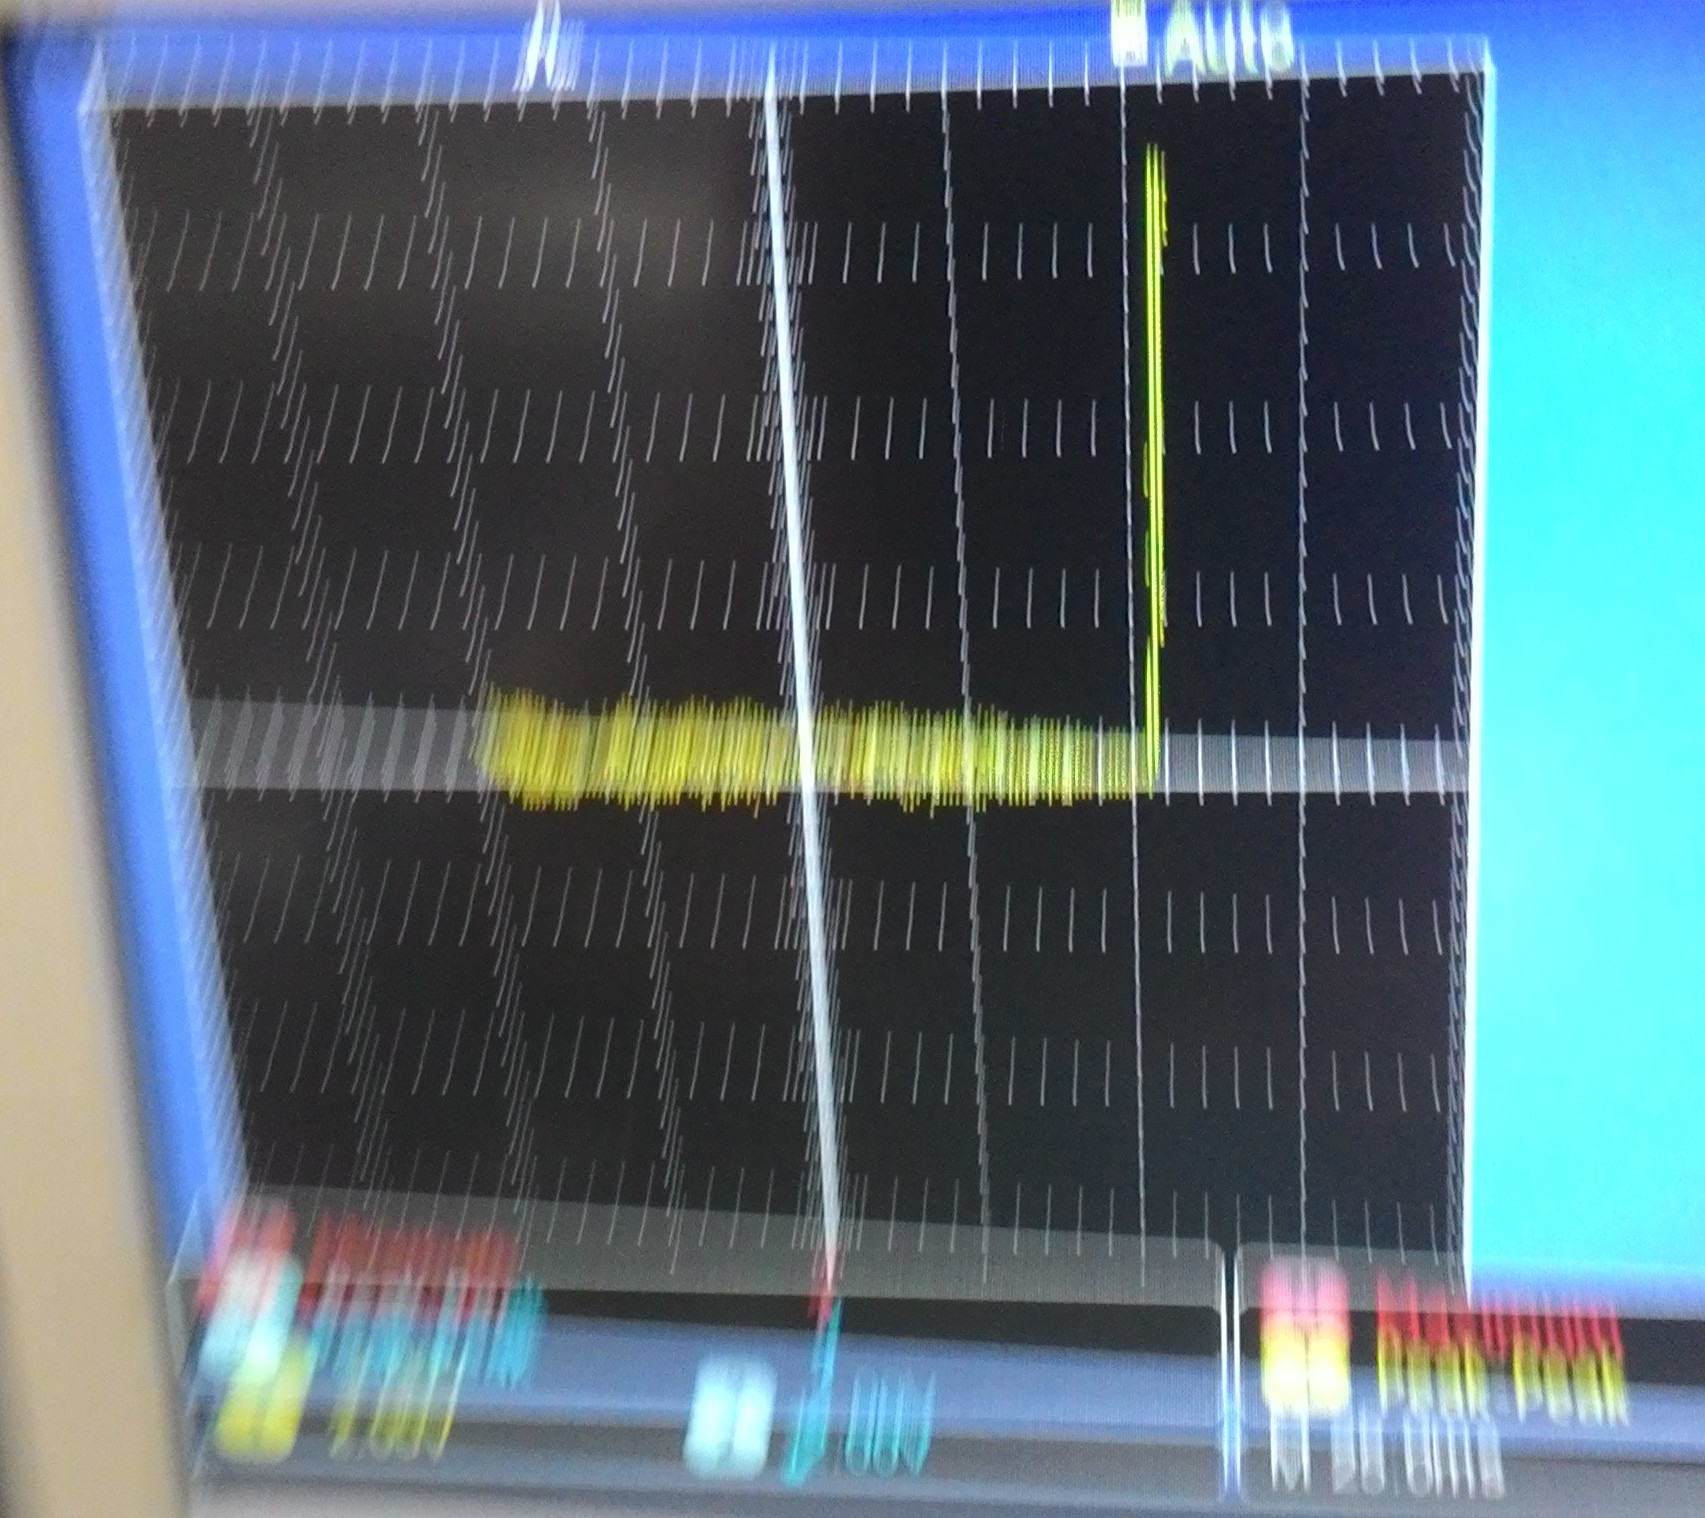
\includegraphics[width=1\textwidth]{img/P2.jpg}
    \caption{Ge}
  \end{subfigure}
  ~
  \begin{subfigure}[b]{0.5\textwidth}
    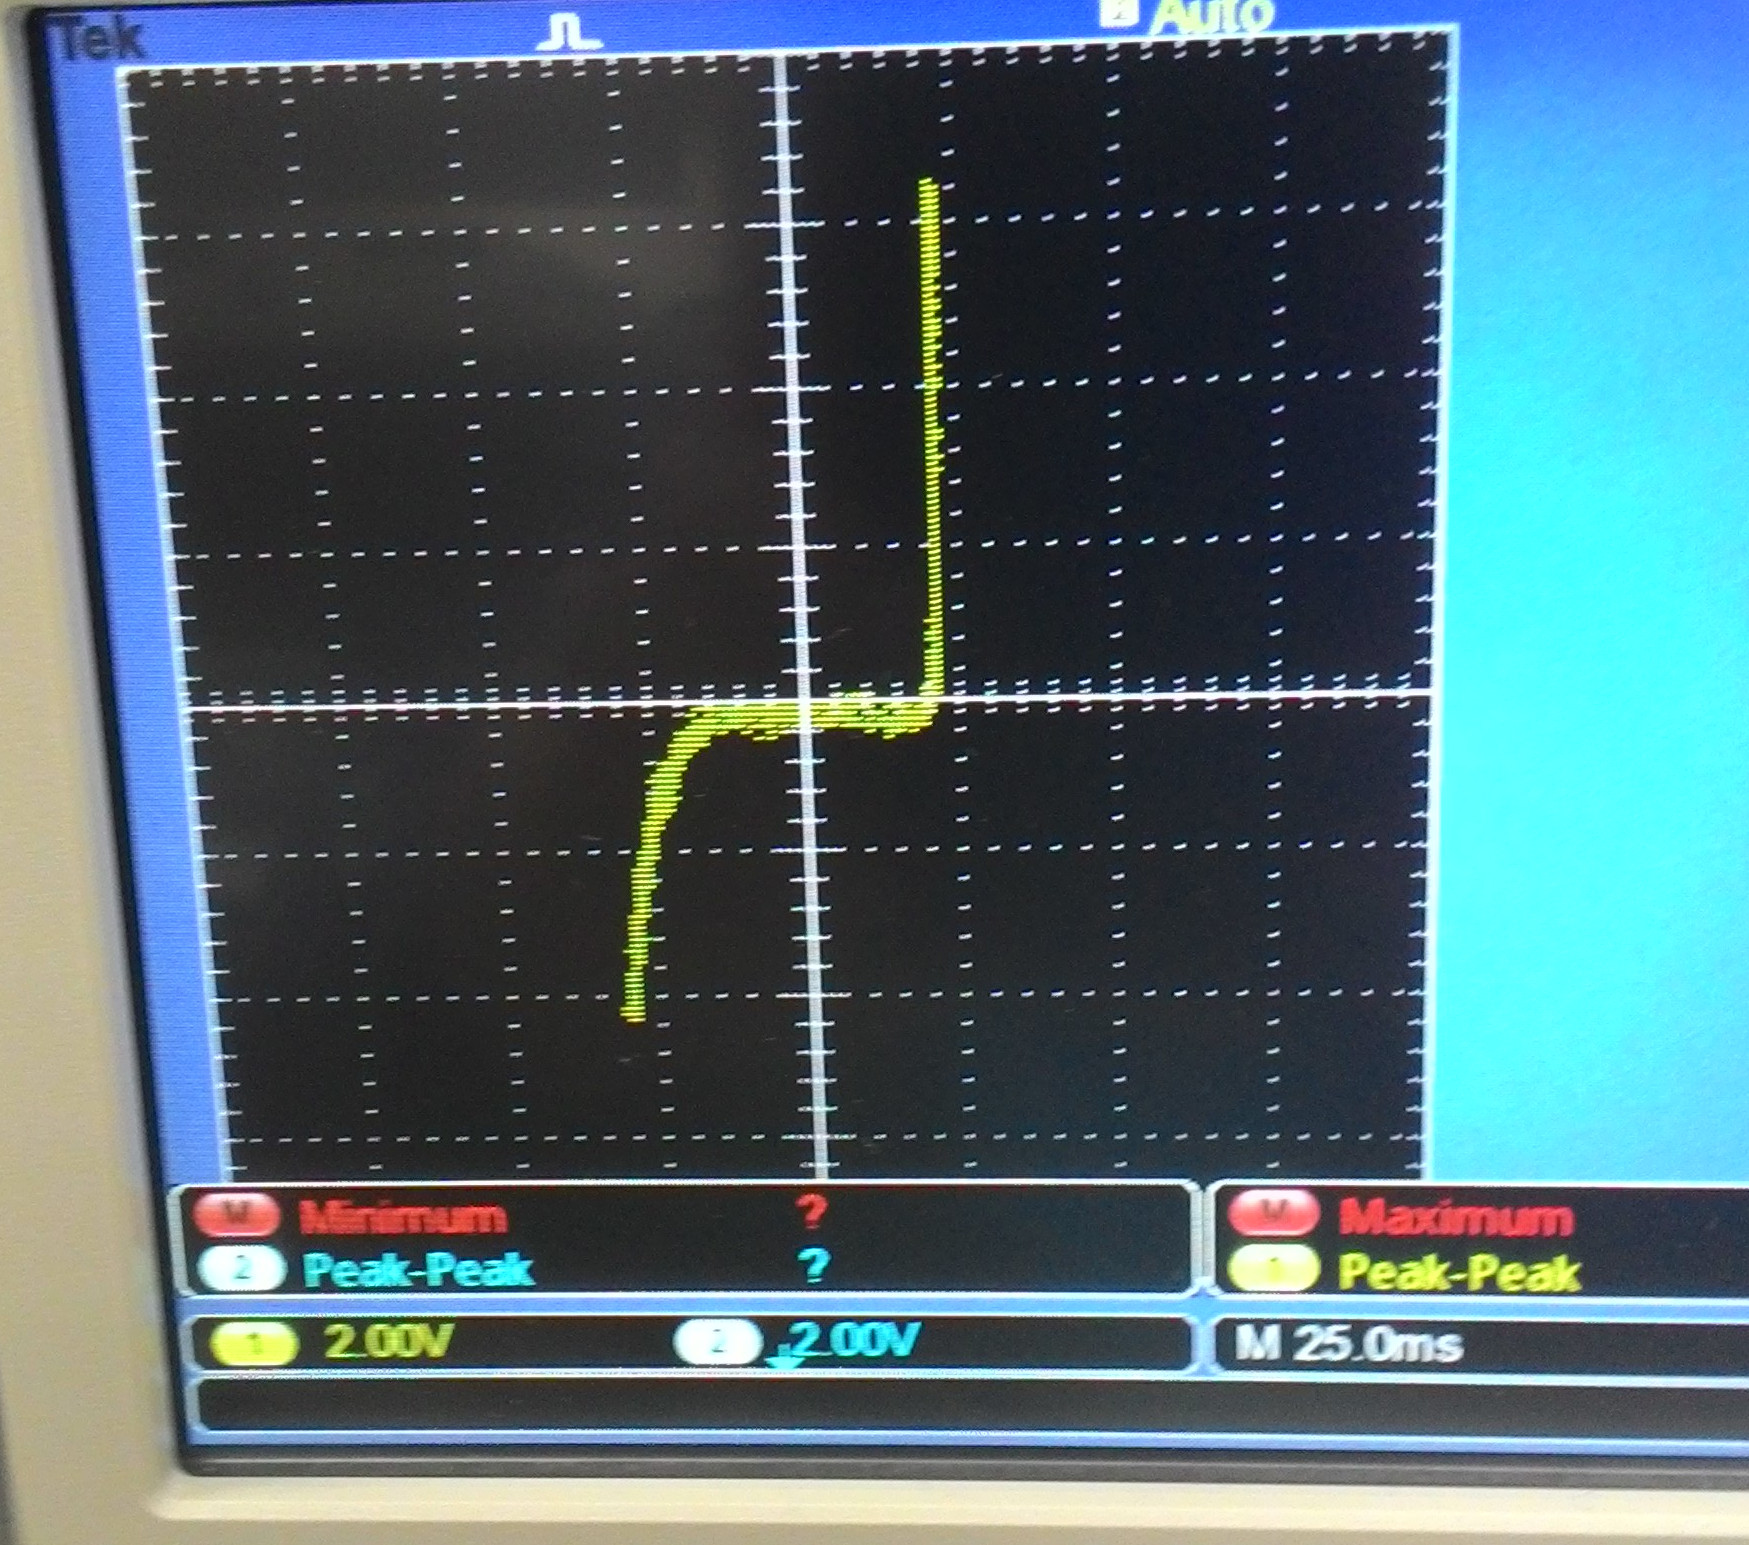
\includegraphics[width=1\textwidth]{img/P3.jpg}
    \caption{Zener}
  \end{subfigure}
\end{figure}

\subsection{\SI{100}\ohm}
\begin{figure}[H]
  \centering
  \begin{subfigure}[b]{0.5\textwidth}
    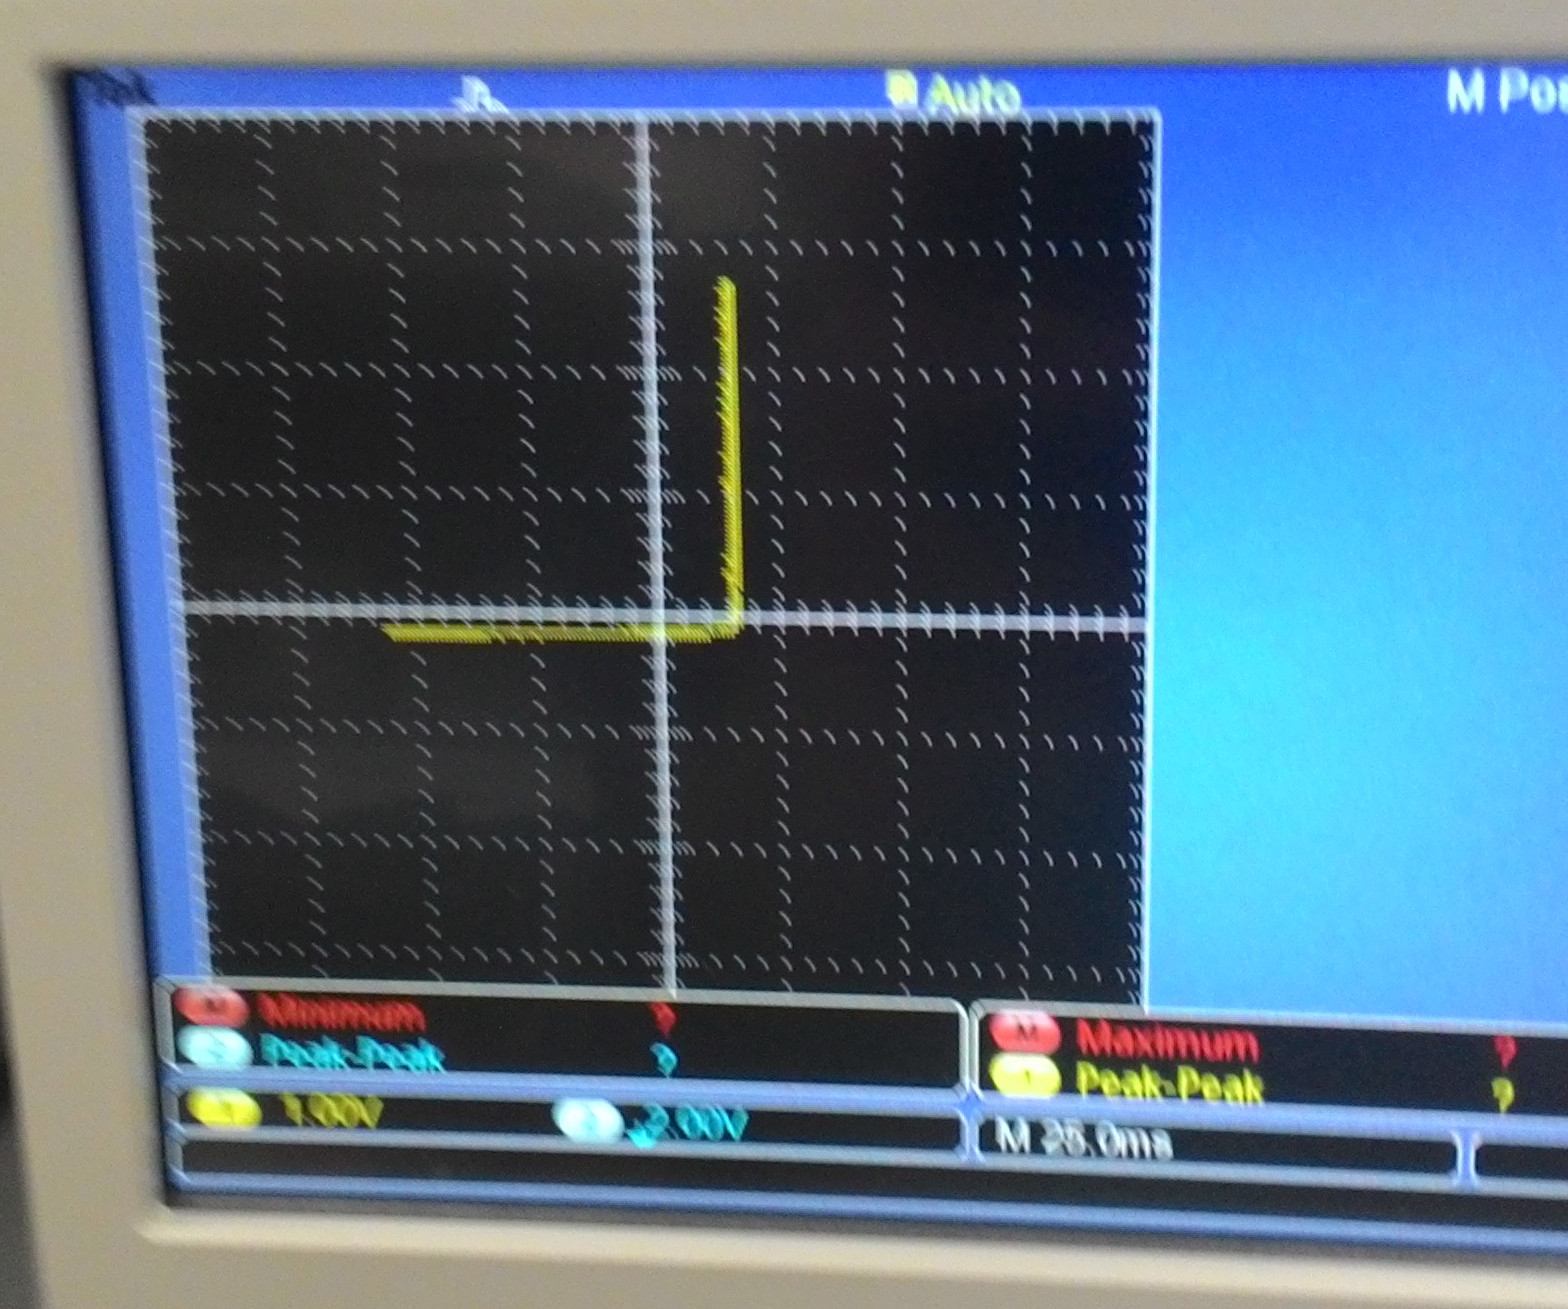
\includegraphics[width=1\textwidth]{img/P4.jpg}
    \caption{Si}
  \end{subfigure}
  \begin{subfigure}[b]{0.5\textwidth}
    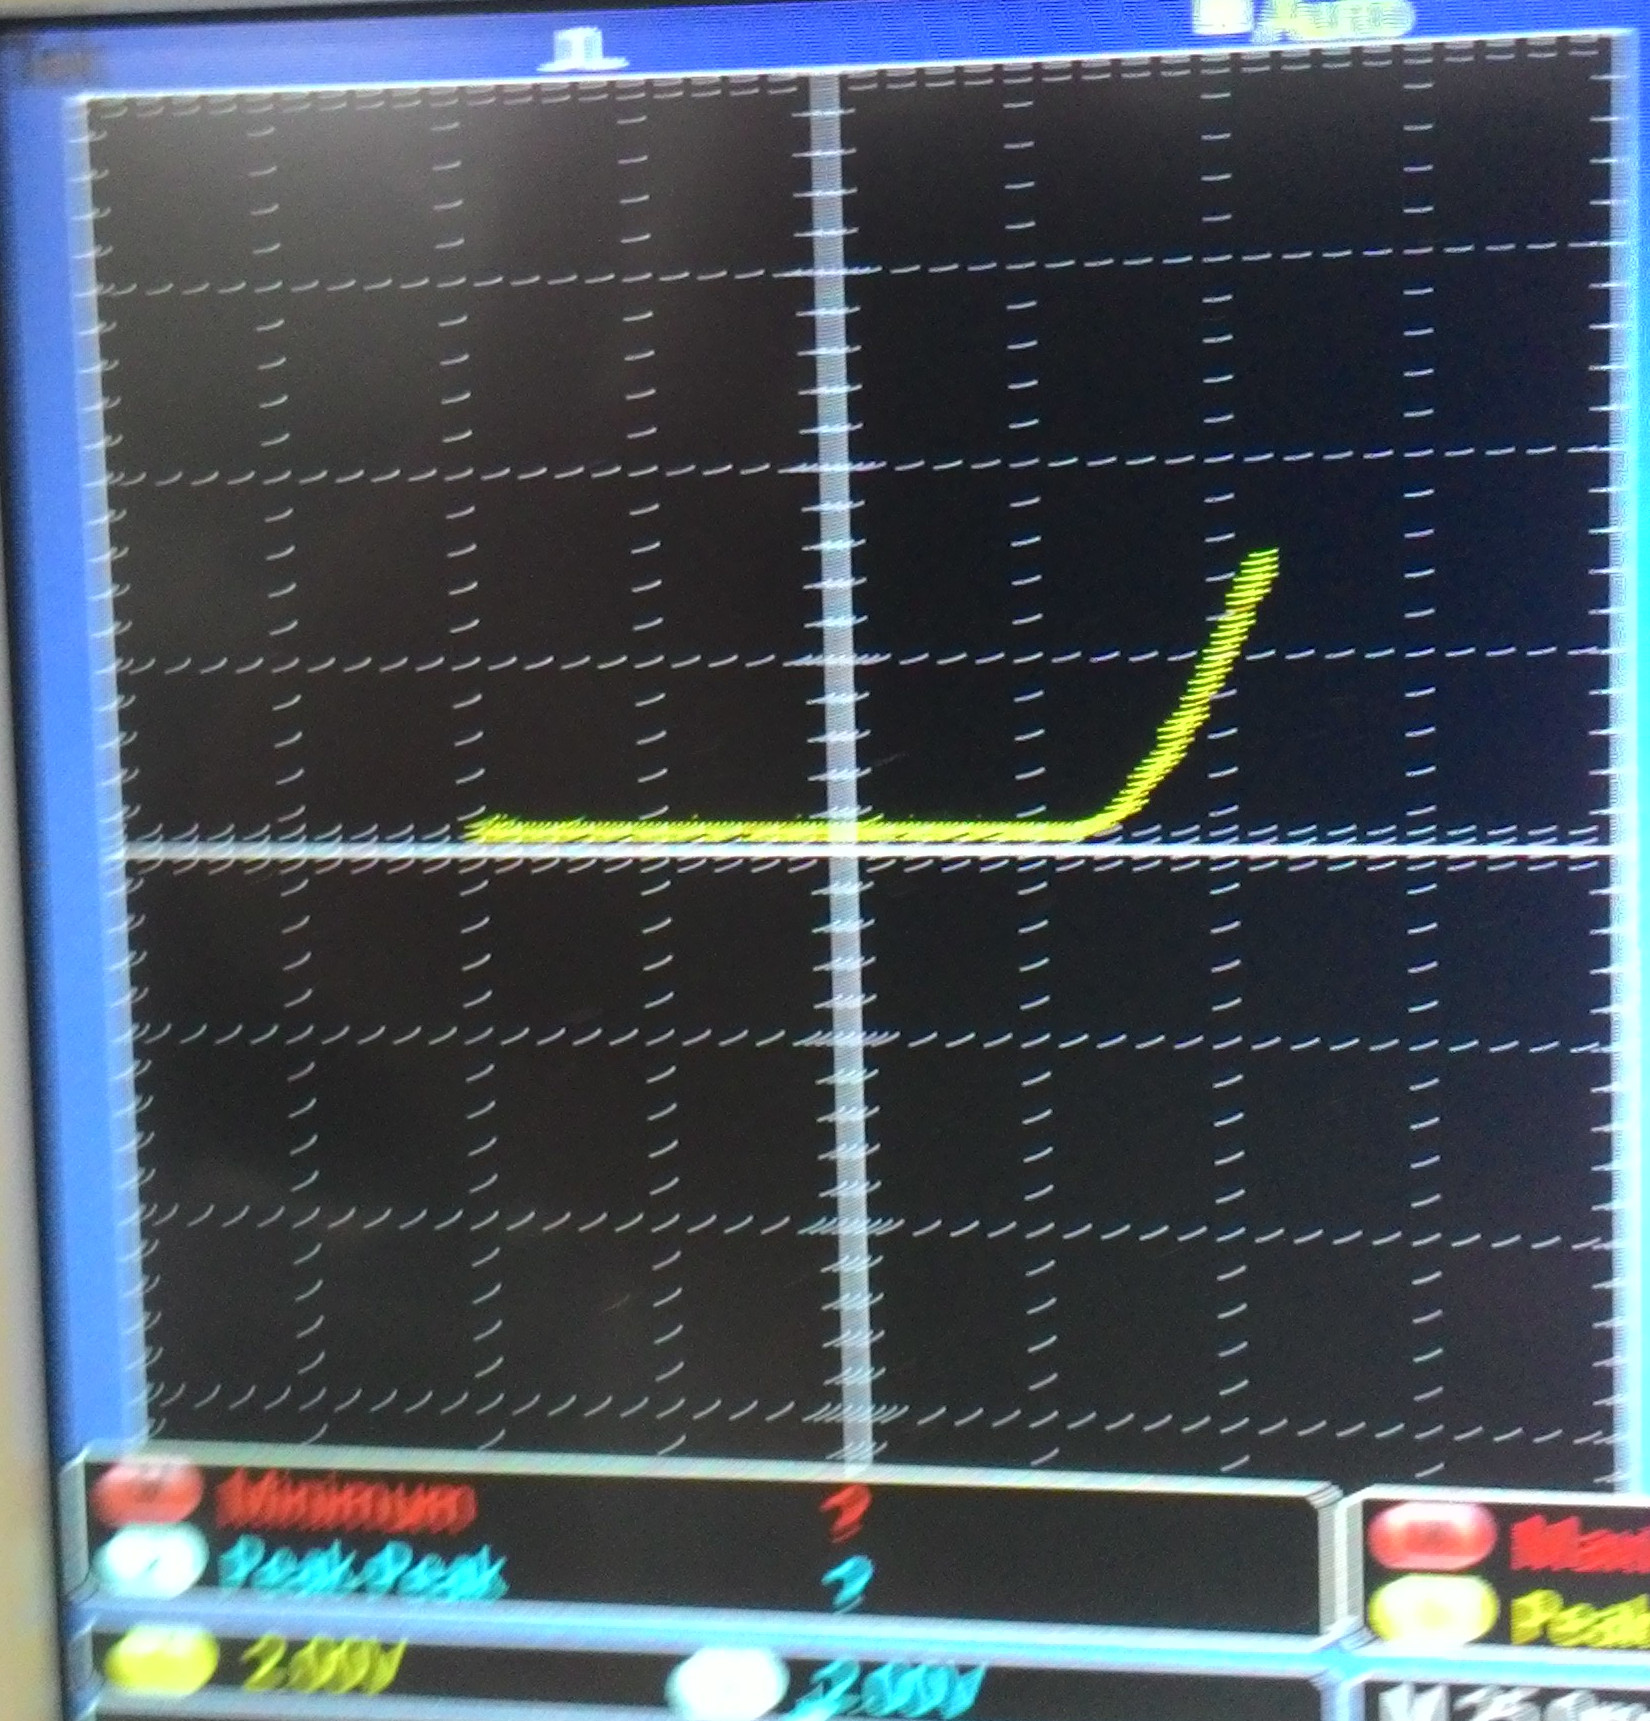
\includegraphics[width=1\textwidth]{img/P5.jpg}
    \caption{Ge}
  \end{subfigure}
  \begin{subfigure}[b]{0.5\textwidth}
    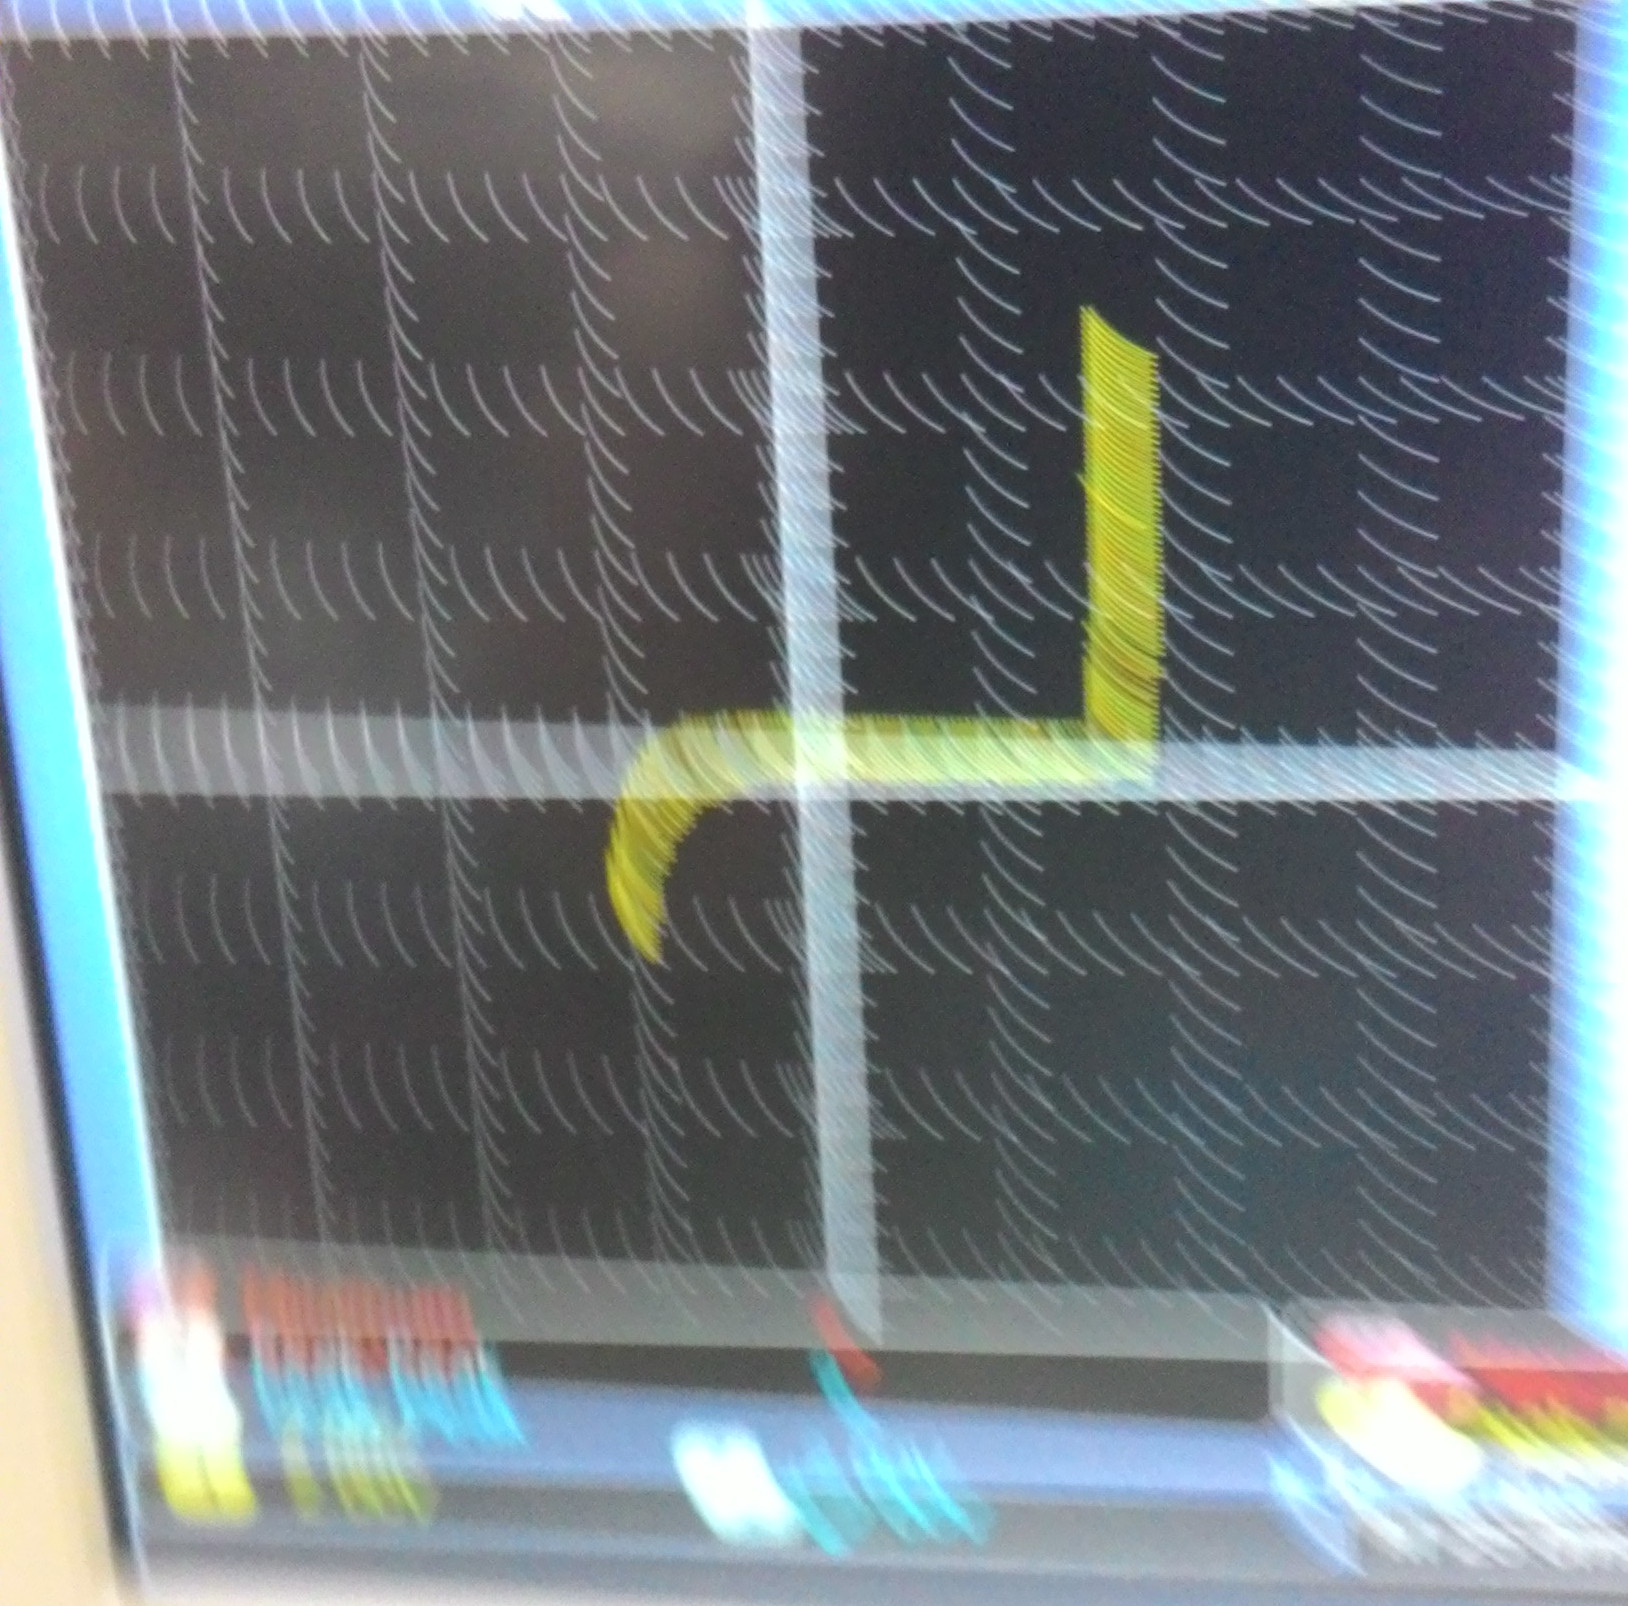
\includegraphics[width=1\textwidth]{img/P6.jpg}
    \caption{Zener}
  \end{subfigure}
\end{figure}


\section{結報問題}

\begin{enumerate}[itemsep=20pt, topsep=10pt]
  \item {\large\bf 如何分辨一未知 Diode 為 Si、Ge 或是 Zener?} \\[10pt]
    答:Zener Diode的breakdown voltage小,容易被觀察到。另外Si的cutoff voltage大概是$\SI{0.7}\V$, Ge是$\SI{0.3}\V$,可再依此分辨出此兩個Diode的差別。 
  \item {\large\bf 試說明 Characteristic Curve 受 frequency、amplitude 影響之現象及原因。} \\[10pt]
    Diode有電容效應,在低頻時不明顯,但在高頻時會受到電容效應充放電的影響,而使得Characteristic Curve分裂成兩條。\\
    Amplitude影響的是電壓峰值,所以當amplitude越大,可測量的電壓範圍也越大,因此Characteristic Curve會往左右擴張。
  \item {\large\bf 電阻使用$\SI{5.1}\kohm$或者$\SI{100}\ohm$有何差異?} \\[10pt]
    基本上Diode的Characteristic I-V Curve不會因此改變,但因為X-Y Mode時我們得到的Y軸並非電流,而是$V_R = I R$,因此$\SI{100}\ohm$的圖形相當於$\SI{5.1}\kohm$的圖形Y軸縮放$5100 / 100$倍的結果。
  \item {\large\bf 試於 X-Y Mode 時,定性敘述 X/Y Channel 相互交換所得之結果。} \\[10pt]
    X, Y交換相當於作變換$(x, y) \mapsto (y, x)$,因此整個圖形會相當於原本的圖形對直線$x = y$作鏡射。但因此實驗Y channel反相,因此原本$(x, y) \mapsto (x, -y)$,交換後$(x, y) \mapsto (y, x) \mapsto (y, -x)$,因此相當於$(x, y) \mapsto (-y, -x)$,也就是對$x = -y$作鏡射。
  \item {\large\bf 對於 Oscilloscope:}
    \begin{enumerate}[label=(\alph*)]
      \item 哪些 Components 應先歸零(Reset)? \\[5pt]
        基本上不要亂調到奇怪的東西,直接按Auto set儀器就幫你調好好的了…
      \item 試述 AC 檔與 DC 檔的差別。\\[5pt]
        AC檔會將訊號的DC component濾掉,只剩下AC部分的波形。
      \item 當波形發生左右漂移時,應如何處置?} \\[5pt]
      直接換一台吧…八成是示波器壞了。硬要說的話把Hold鈕拉起來在停止的波形上做觀察。
    \end{enumerate}
  \item {\large\bf 對於 Probe:}
    \begin{enumerate}[label=(\alph*)]
      \item 棒上的 X1、X10,對波形有何影響?\\[5pt]
      $\times 1$測到的是實際的電壓,而$\times 10$測到的是$1/10$倍的電壓。\\
      \item 在此實驗中,可否將兩 Channel 的正負兩端互換?為什麼?\\[5pt]
      不可,因為示波器兩個Channel的負端都會接地,因此兩端必須接在同一點。
    \end{enmerate}
\end{enumerate}

\section{心得}
這次的實驗好像不少人的實驗器材有一點問題,像我旁邊的同學他電路接的好好的,不知道為什麼示波器上就是會有雜訊。後來他把訊號產生器換成我座位的那一台,雜訊瞬間少了一半,再把示波器換成我的那一台就完全好了。不知道如果考試的時後這樣有沒有什麼補救的方法。
\end{document}

